\section{Methods}
\subsection{U-Net}
\subsubsection{Motivation}
Here we explain why we choose U-Net as our first and baseline method to experiment with. Published in \cite{unet}, it has been cited over 10000 times and widely used as a benchmark in medical image segementation. Based on U-Net, many vairations are designed to pursue better performance, as we will see in later parts. Nevertheless, U-Net itself was a big breakthrough at its publish time, and it is very beneficial to study with its netwrok structure.

\subsubsection{Detailed Description}
Image segementation has long been a major task in computer vision, where the input is an image and the expected output is the mask of image\textemdash where all pixels belonging to the same object are labeled out (See Figure~\ref{fig:sege}). 
\begin{figure}[!htpb]
    \centering
    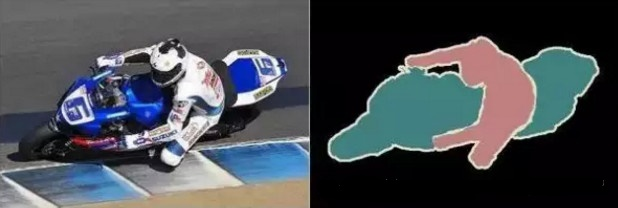
\includegraphics[scale=0.3]{figuras/segementation.jpg}
    \caption{An illustration of the goal of iamge segementation.}
    \label{fig:sege}
\end{figure}

The first try to combine deep learning methods with this task is Fully Convolutional Networks by \cite{FCN}, which became a milestone. We know that in traditional CNN, the feature dimension is decreased by convolution and pooling operations, and the reception region change from local to global gradually as the image propagate through the network. This makes it difficult to do segementation, as we have to restore the size of image. FCN uses reversed convolution and upsampling operation to restore image size, and conduct pixel-level classification.
\begin{figure}[!htpb]
    \centering
    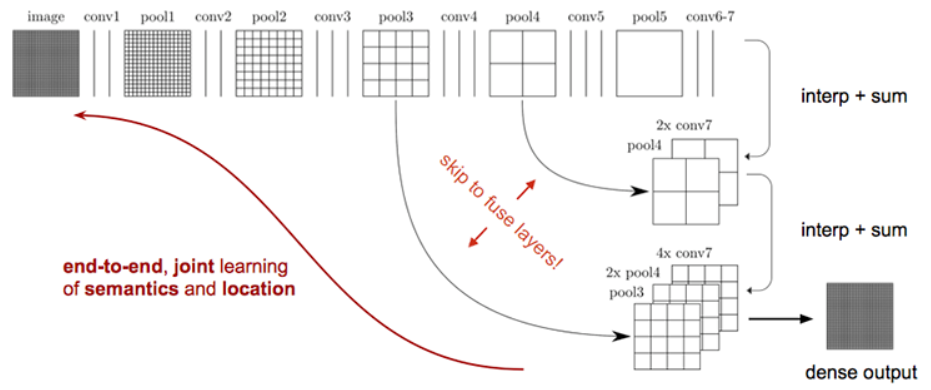
\includegraphics[scale=0.3]{figuras/FCN.PNG}
    \caption{Structure of Fully Convolutional Network, where it fuses pool4, pool3 and feature map to concate features.}
    \label{fig:fcn}
\end{figure}

However, FCN is not good at image details (see Figure~\ref{fig:fcnd}). The result is often blurred and smooth, thus not suitable for medical image segementation, where we especailly care about edges and details in the image, in case the doctors make wrong diagnosis. So there came U-Net, which imporve based on FCN. 

\begin{figure}[!htpb]
    \centering
    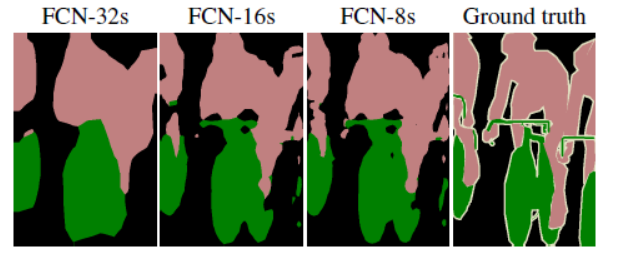
\includegraphics[scale=0.5]{figuras/FCNdetail.PNG}
    \caption{Some results of FCN compared with the ground truth. Details of the cycling man isn't very good.}
    \label{fig:fcnd}
\end{figure}

Figure~\ref{fig:unets} shows the structure of U-Net. It uses many feature channels to allow features containing more information on the texture of original image to propagate between high-resolution layers. And it is specaily designed for medical tasks, where it is very difficult to separate the connected same-category cells. The authors proposed weighted loss function, where it gives the ground truth of connected cells more consideration. U-Net can perform well on small datasets like ISBI challenge, and does not require demanding GPU memory. Of course, data augmentation needs to be done before training.

\begin{figure}[!htpb]
    \centering
    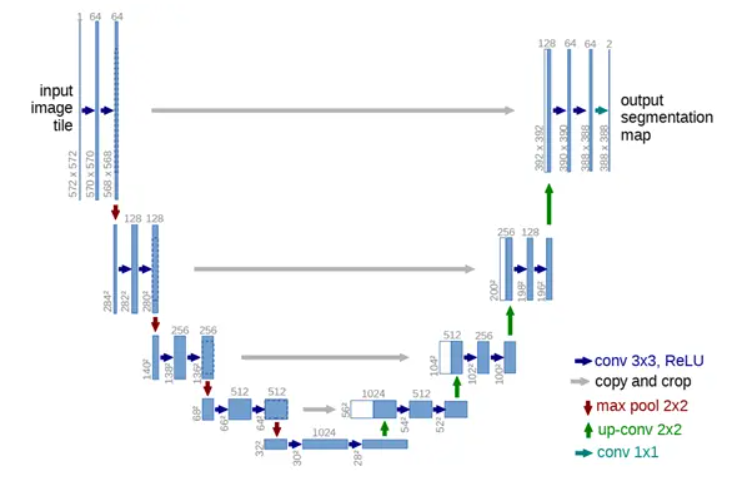
\includegraphics[scale=0.4]{figuras/unet.PNG}
    \caption{Sructure of U-Net. It looks like the character `U'. }
    \label{fig:unets}
\end{figure}